% ============================================================
% CAPÍTULO 3: REQUISITOS FUNCIONALES
% ============================================================
\section{Requisitos funcionales}
\label{sec:requisitos_funcionales}

Esta sección describe las interfaces del sistema y los casos de uso que representan el comportamiento externo de AnxioTest, siguiendo la notación de Cockburn. Se incluyen dos niveles de casos de uso: Nivel 0 (visión estratégica) y Nivel 1 (objetivos del usuario). Cada caso de uso se detalla con su flujo normal, excepciones y condiciones.

\subsection{Interfaces externas}
\label{sec:interfaces_externas}

\subsubsection{Interfaz de usuario}
\label{sec:interfaz_usuario}

El sistema AnxioTest presenta una interfaz minimalista, con tipografía grande, botones prominentes y colores de alto contraste, diseñada específicamente para facilitar su uso por parte de adultos mayores y personas con poca familiaridad tecnológica. A continuación se describen las pantallas principales:

\begin{longtable}{p{0.22\linewidth} p{0.73\linewidth}}
\toprule
\rowcolor{tableheader!20}
\textbf{Pantalla} & \textbf{Descripción} \\
\midrule
\endfirsthead
\rowcolor{tableheader!20}
\textbf{Pantalla} & \textbf{Descripción} \\
\midrule
\endhead
\bottomrule
\endfoot
\textbf{Página de inicio}
  & Pantalla de bienvenida con el nombre del sistema, una breve descripción de su propósito, un botón destacado para iniciar la evaluación, el selector de temas y la advertencia de uso clínico. \\
\textbf{Selección de pruebas}
  & Pantalla que muestra dos tarjetas visuales para PHQ-9 y BAI, con descripciones breves de cada cuestionario y botones para iniciar. Incluye botón para regresar al inicio. \\
\textbf{Cuestionario}
  & Pantalla que presenta una pregunta a la vez con cuatro opciones de respuesta. Muestra el progreso (número de pregunta y porcentaje) y botones de navegación (Anterior, Siguiente, Cancelar). Incluye funcionalidad de lectura por voz (TTS) y ayuda contextual. \\
\textbf{Resultados}
  & Pantalla que muestra el puntaje obtenido, la categoría de severidad (con etiqueta amigable), un mensaje interpretativo personalizado, recomendaciones prácticas, y botones para repetir el cuestionario o volver al inicio. \\
\textbf{Selector de temas}
  & Componente en el encabezado que permite al usuario elegir entre diferentes esquemas de colores predefinidos (Claro, Oscuro, Alto Contraste). \\
\bottomrule
\caption{Descripción textual de las interfaces de usuario}
\label{tab:interfaces_ui}
\end{longtable}

Las siguientes figuras ilustran el aspecto visual de cada una de las pantallas descritas anteriormente:

% ====== FIGURA 1: PÁGINA DE INICIO ======
\begin{figure}[H]
  \centering
  % ====== CAMBIA EL NOMBRE DEL ARCHIVO POR EL TUYO ======
  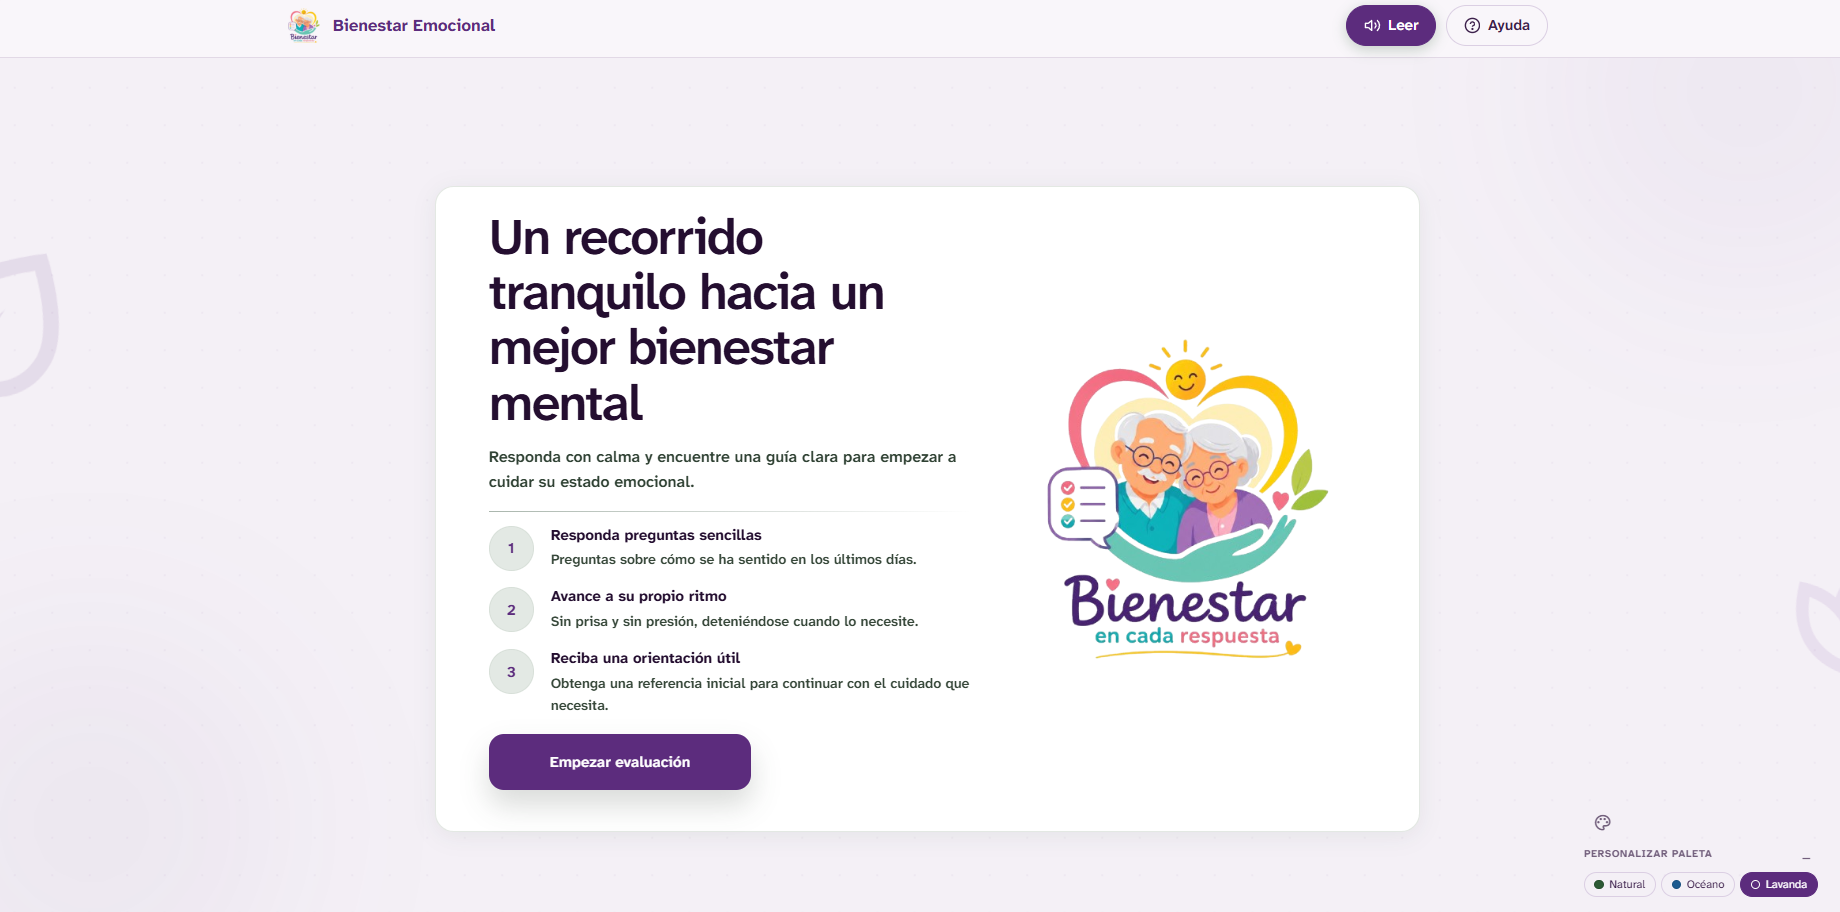
\includegraphics[width=0.85\textwidth]{Portada.png}
  \caption{Página de inicio de AnxioTest.}
  \label{fig:ui_inicio}
\end{figure}

% ====== FIGURA 2: SELECCIÓN DE PRUEBAS ======
\begin{figure}[H]
  \centering
  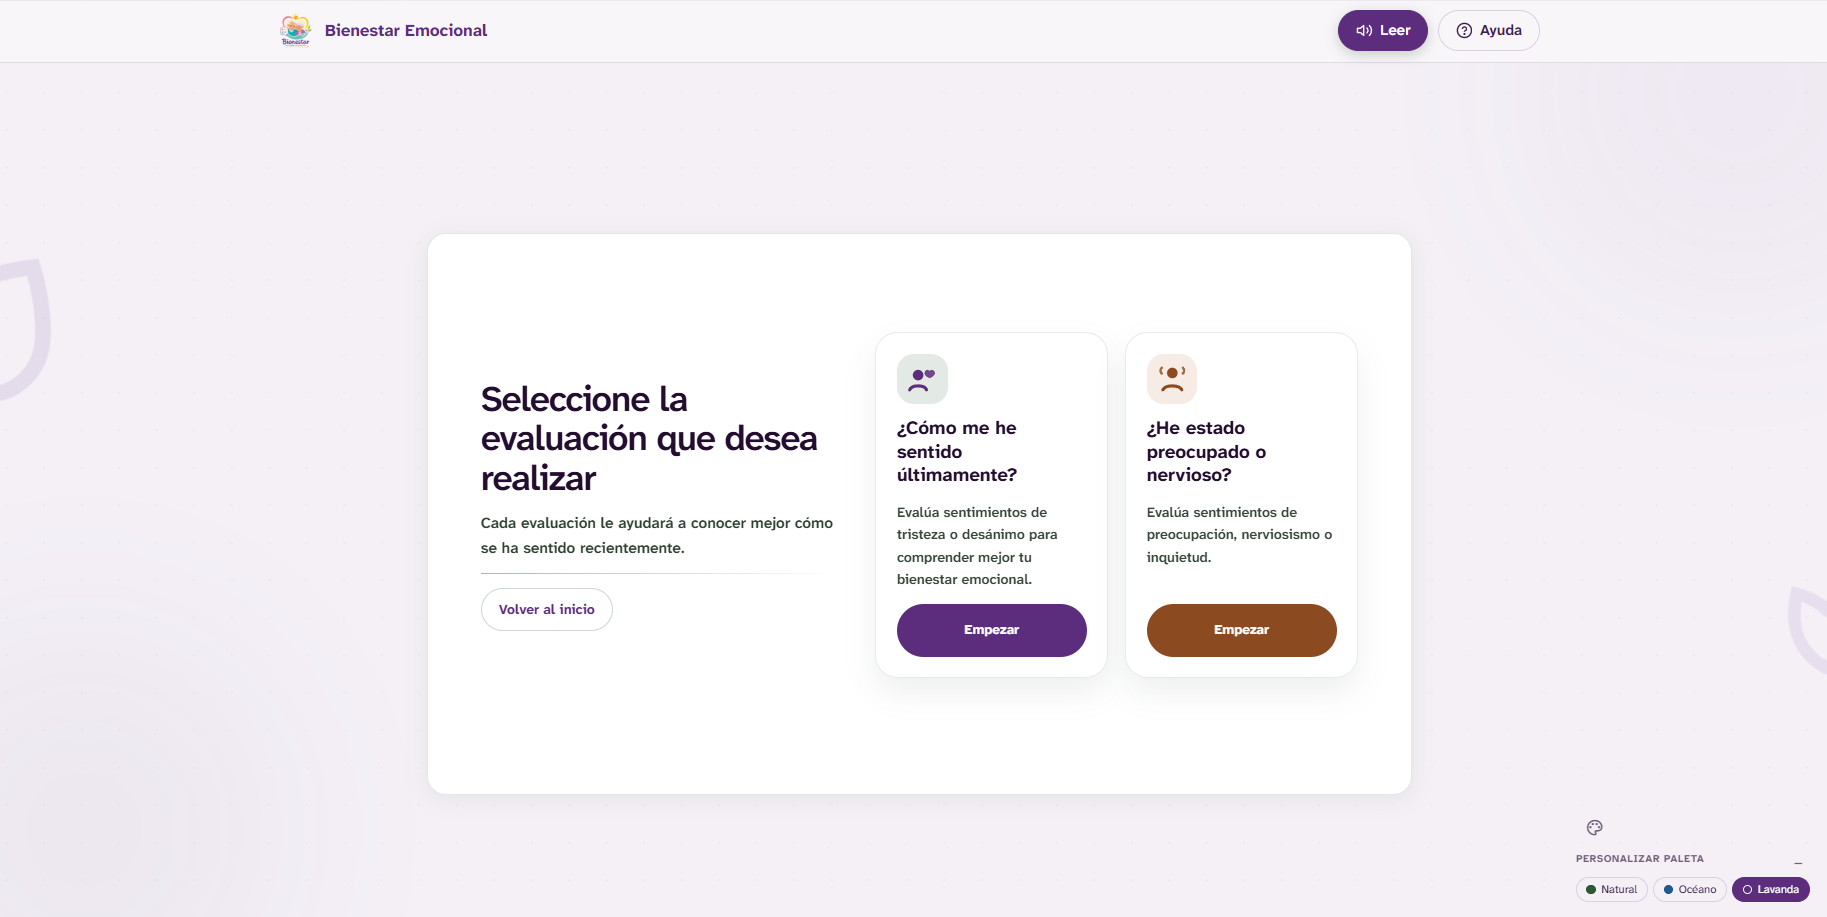
\includegraphics[width=0.85\textwidth]{Eleccion.png}
  \caption{Página de selección de pruebas (PHQ-9 y BAI).}
  \label{fig:ui_seleccion}
\end{figure}

% ====== FIGURA 3: CUESTIONARIO ======
\begin{figure}[H]
  \centering
  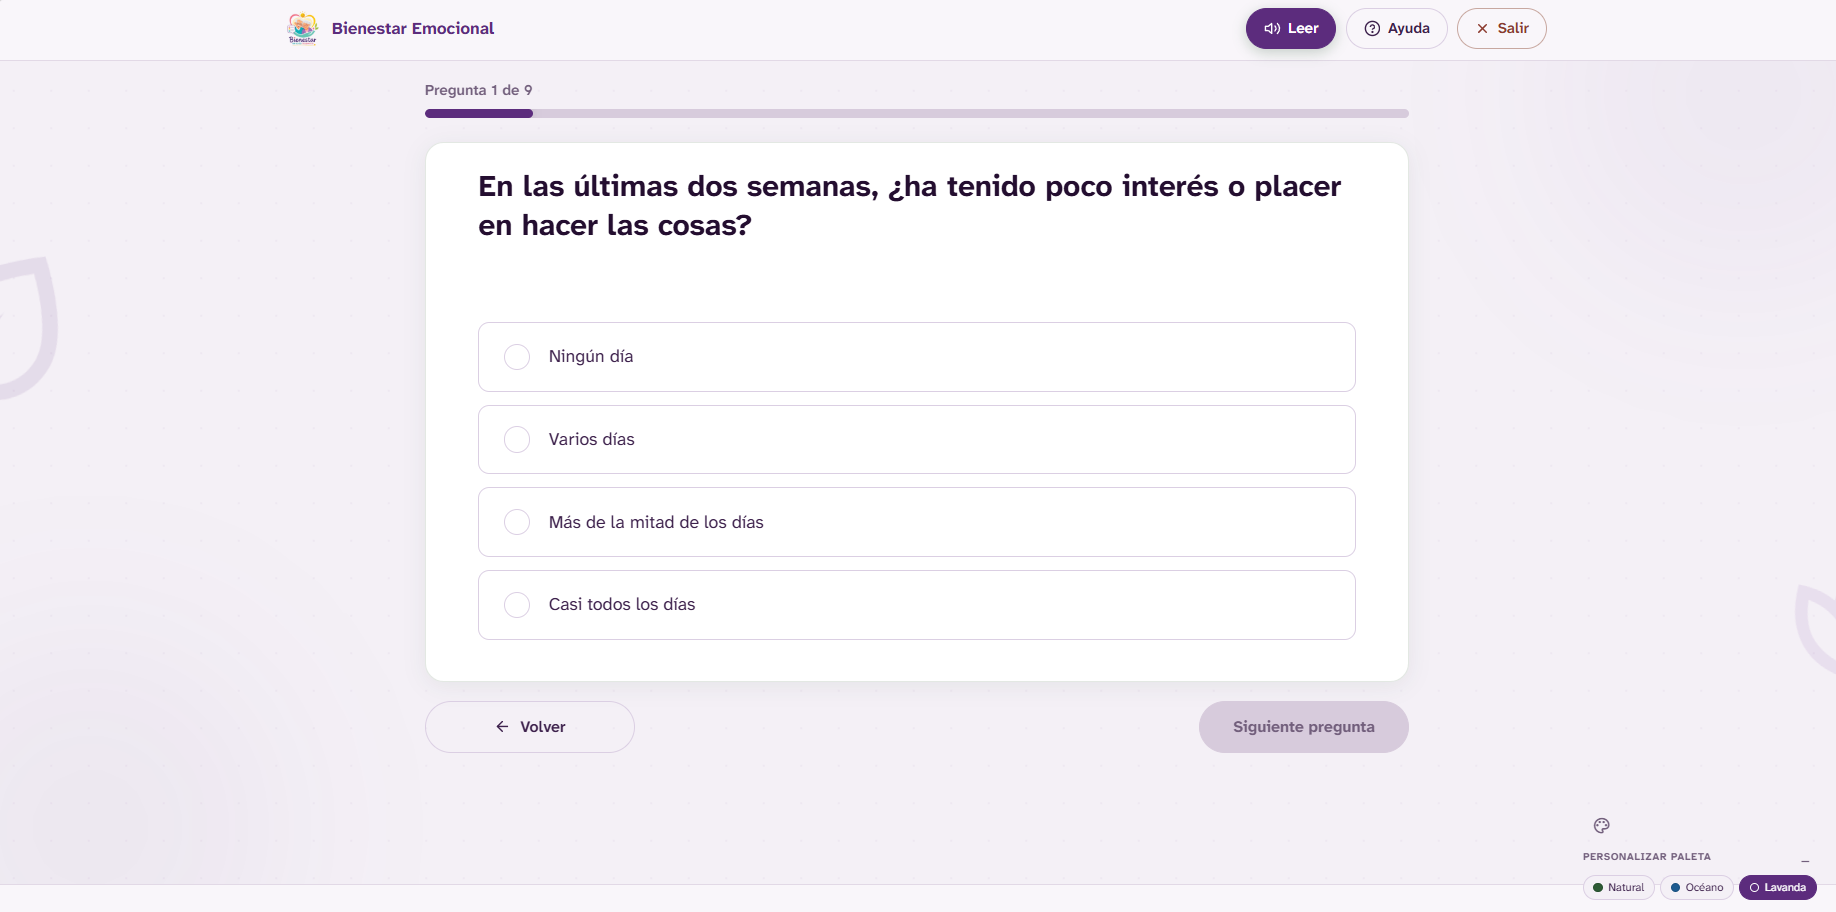
\includegraphics[width=0.85\textwidth]{cuestionario.png}
  \caption{Ejecución del cuestionario: pregunta secuencial, opciones de respuesta y botón de voz (TTS).}
  \label{fig:ui_cuestionario}
\end{figure}

% ====== FIGURA 4: RESULTADOS ======
\begin{figure}[H]
  \centering
  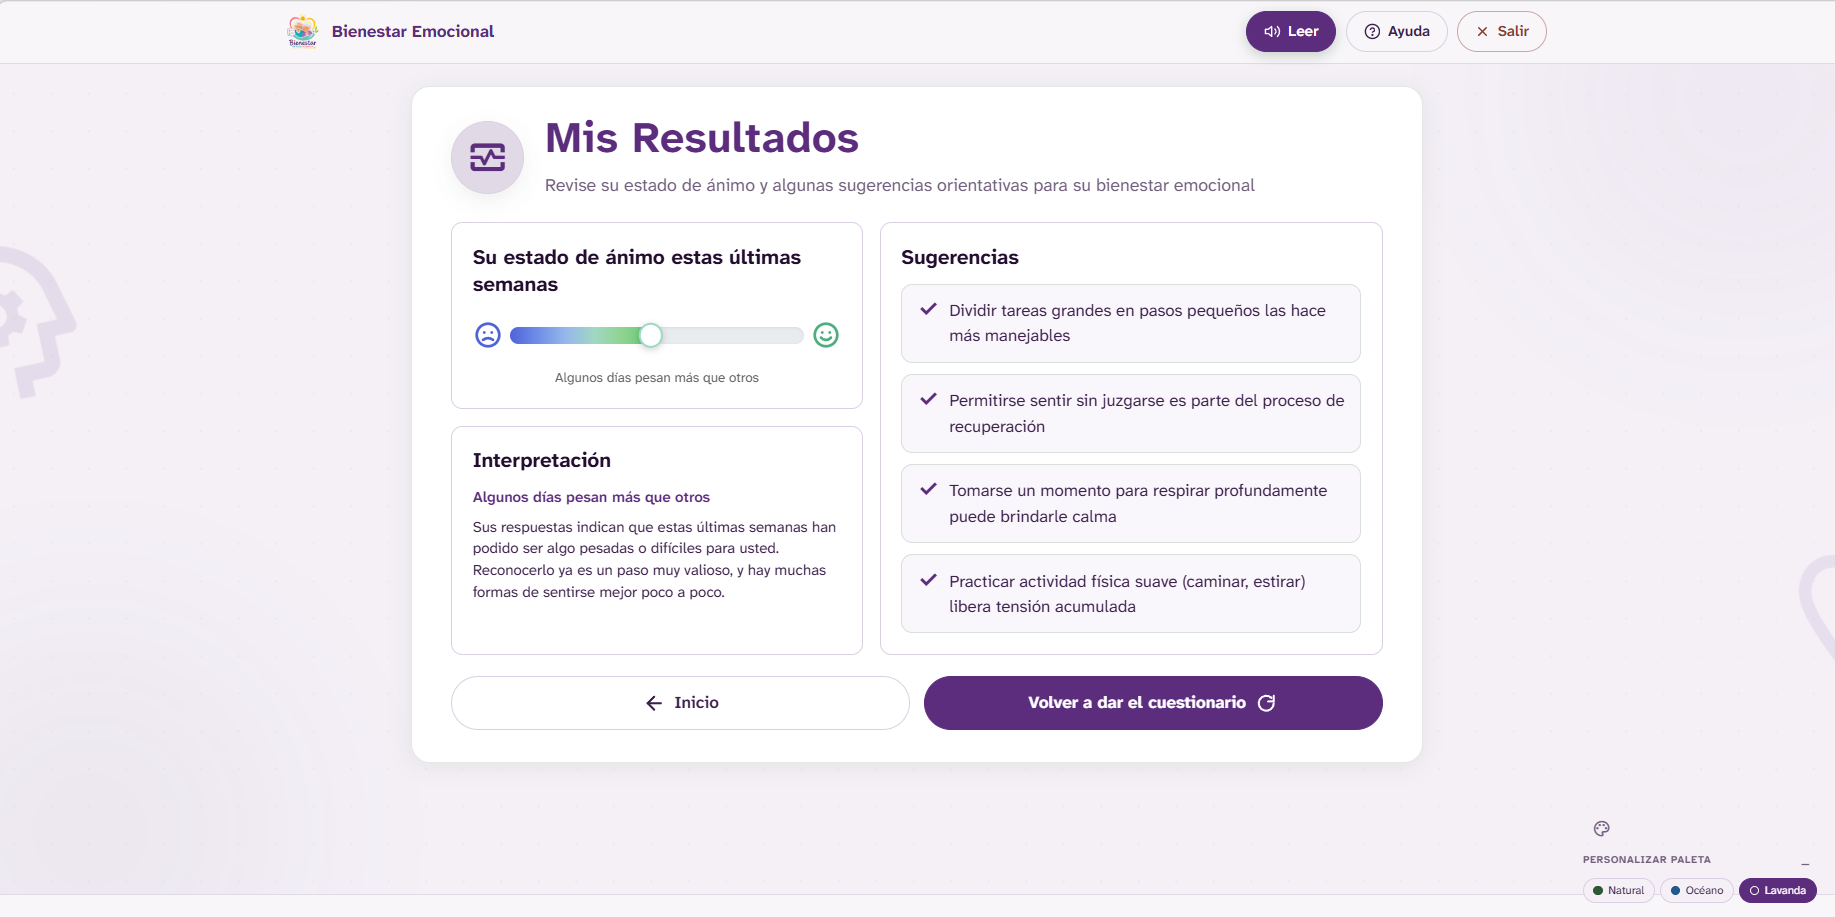
\includegraphics[width=0.85\textwidth]{resultados.png}
  \caption{Página de resultados con puntaje, categoría amigable y recomendaciones.}
  \label{fig:ui_resultados}
\end{figure}

% ====== FIGURA 5: SELECTOR DE TEMAS (OPCIONAL) ======
\begin{figure}[H]
  \centering
  \begin{subfigure}[b]{0.3\textwidth}
    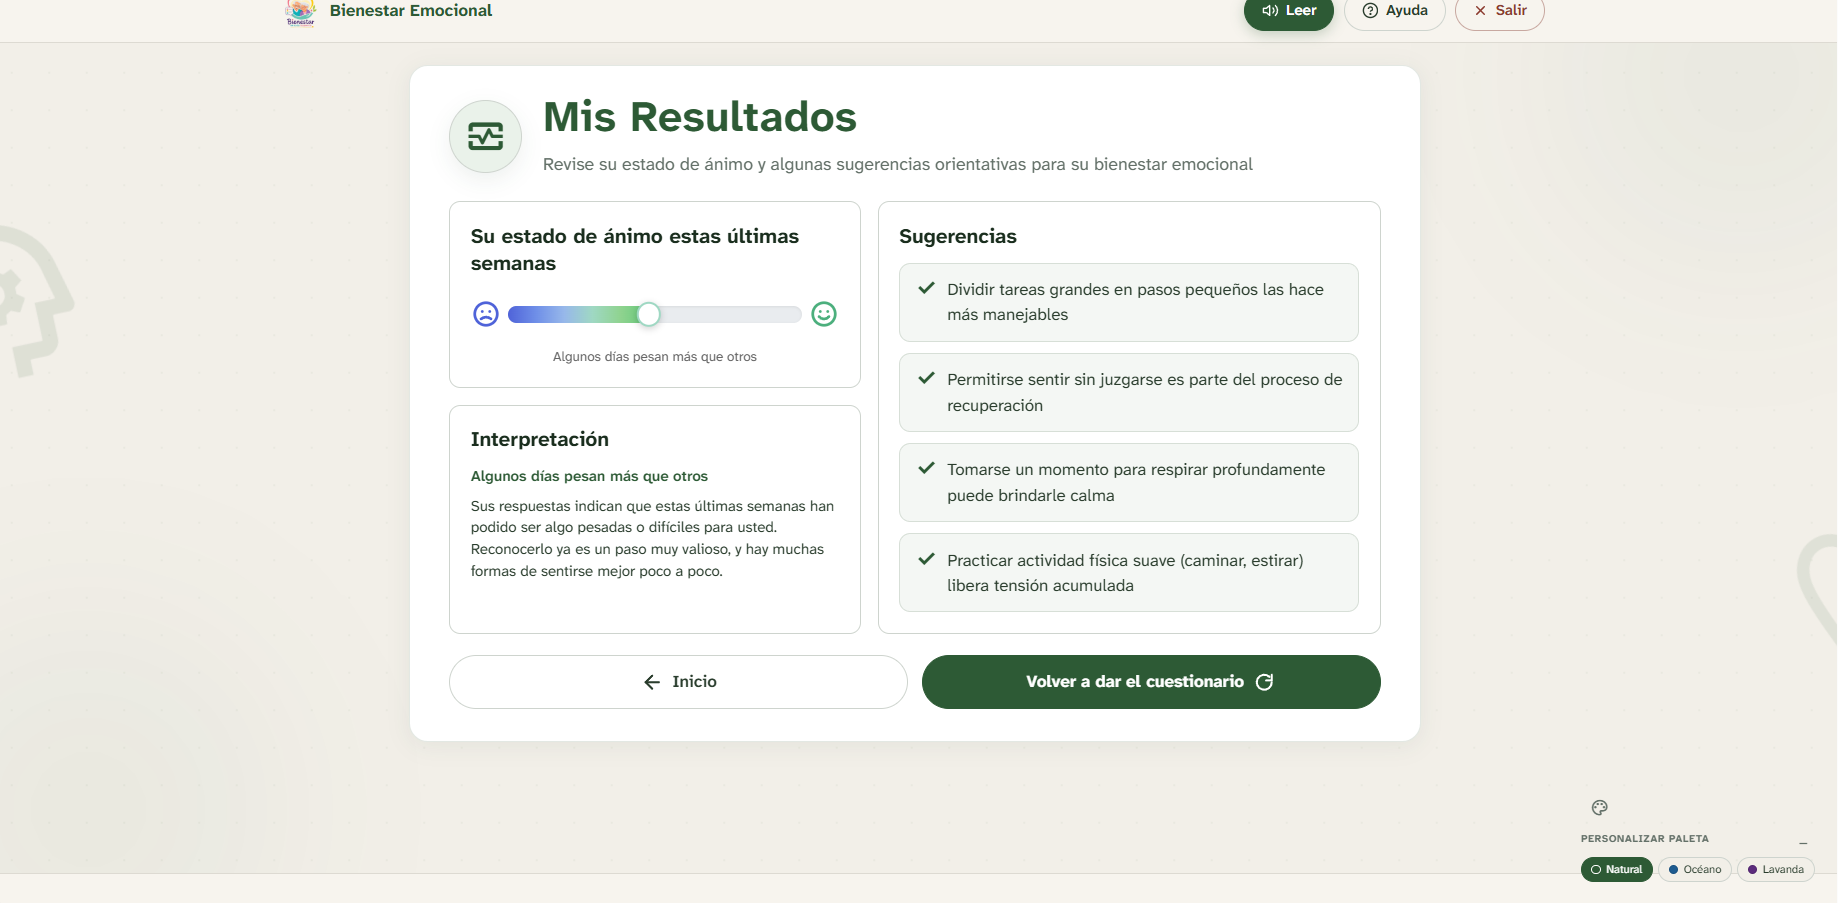
\includegraphics[width=\linewidth]{tema1.png}
    \caption{Tema Claro}
    \label{fig:ui_claro}
  \end{subfigure}
  \hfill
  \begin{subfigure}[b]{0.3\textwidth}
    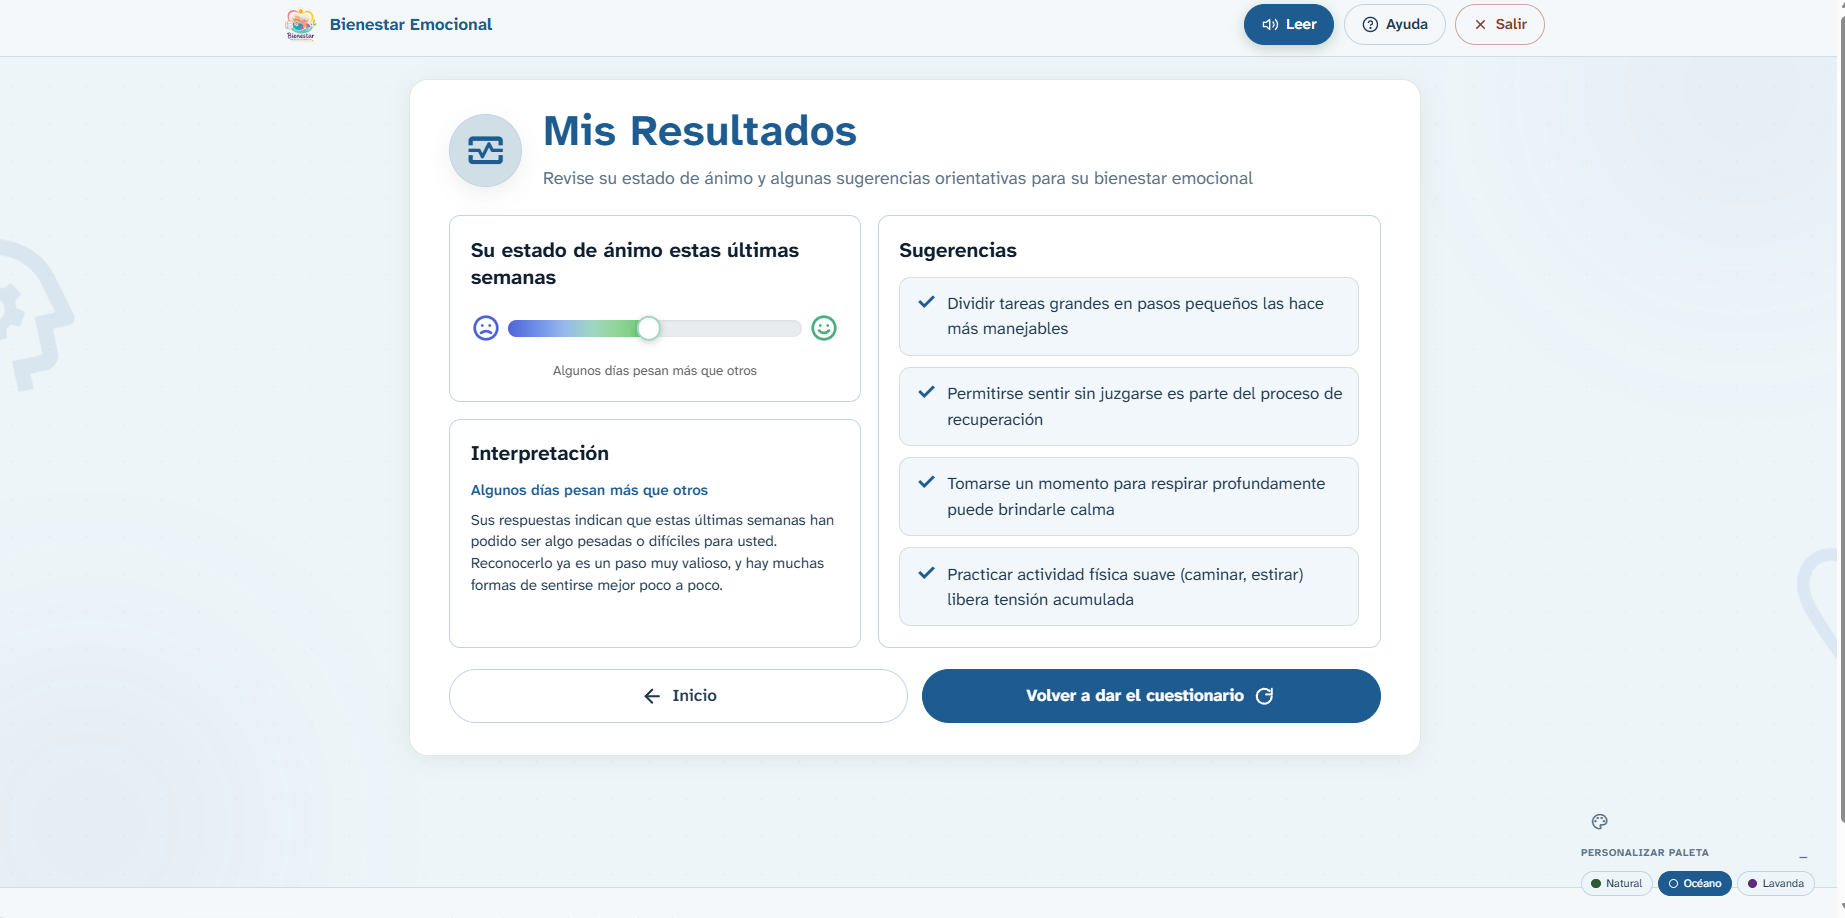
\includegraphics[width=\linewidth]{tema2.png}
    \caption{Tema Oscuro}
    \label{fig:ui_oscuro}
  \end{subfigure}
  \hfill
  \begin{subfigure}[b]{0.3\textwidth}
    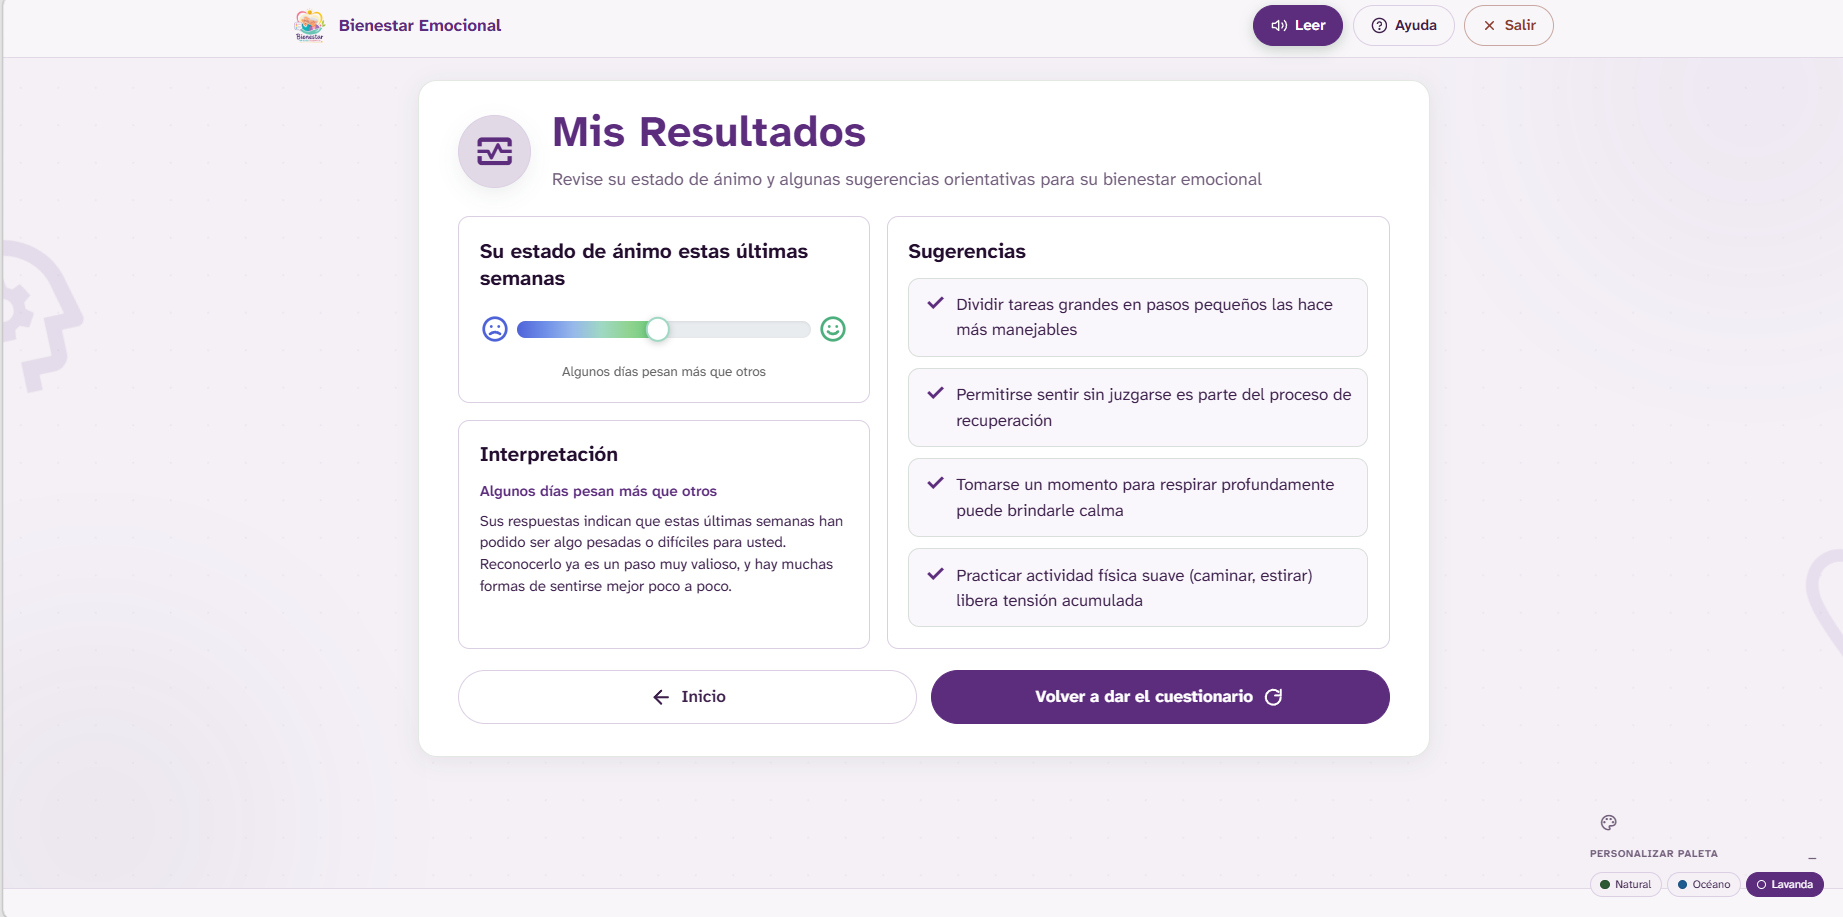
\includegraphics[width=\linewidth]{tema3.png}
    \caption{Tema Alto Contraste}
    \label{fig:ui_alto_contraste}
  \end{subfigure}
  \caption{Interfaces del sistema según el tema visual seleccionado: Claro, Oscuro y Alto Contraste.}
  \label{fig:ui_temas}
\end{figure}

Todos los elementos interactivos incluyen atributos ARIA y son navegables mediante teclado, tal como se especifica en los requisitos RF-24 y RF-25, y en los requisitos no funcionales de accesibilidad.

\subsubsection{Interfaz software}
\label{sec:interfaz_software}

\begin{longtable}{p{0.25\linewidth} p{0.70\linewidth}}
\toprule
\rowcolor{tableheader!20}
\textbf{Componente} & \textbf{Descripción} \\
\midrule
\endfirsthead
\rowcolor{tableheader!20}
\textbf{Componente} & \textbf{Descripción} \\
\midrule
\endhead
\bottomrule
\endfoot
\texttt{sessionStorage} & Almacenamiento temporal para transferir resultados de evaluación entre páginas. Los datos se eliminan al cerrar la pestaña del navegador. \\
\texttt{localStorage}   & Almacenamiento persistente para guardar la preferencia de tema visual del usuario. Los datos permanecen entre sesiones. \\
\textbf{Google Fonts}   & Fuentes tipográficas cargadas de forma remota para garantizar una presentación visual consistente. \\
\textbf{Bibliotecas de iconos} & Recursos externos de iconos utilizados para mejorar la experiencia visual. \\
\textbf{API TTS}        & Interfaz del navegador (\texttt{SpeechSynthesis}) para lectura de preguntas en voz alta. \\
\bottomrule
\caption{Interfaces software}
\label{tab:interfaces_sw}
\end{longtable}

\subsubsection{Interfaz hardware}
\label{sec:interfaz_hardware}

El sistema se ejecuta en navegadores modernos y no requiere hardware especializado. Los requisitos mínimos de hardware son:

\begin{itemize}
  \item Dispositivo con capacidad para ejecutar un navegador moderno (ordenador personal, portátil, tablet o smartphone).
  \item Conexión a Internet para cargar recursos externos (fuentes, iconos).
  \item Altavoces o auriculares para la funcionalidad de lectura por voz.
  \item Pantalla con resolución mínima de 320\,px de ancho para compatibilidad con dispositivos móviles.
\end{itemize}

\subsection{Diagrama de Casos de Uso – Nivel 0}
\label{sec:dcu_nivel0}

\begin{figure}[H]
  \centering
  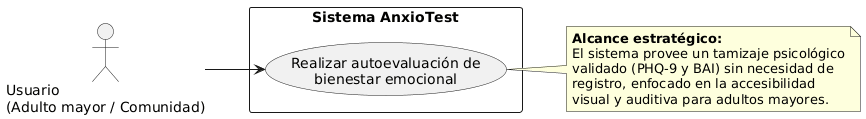
\includegraphics[width=0.8\textwidth]{nivel0-vincu.png}
  \caption{Diagrama de casos de uso – Nivel 0 (visión estratégica).}
  \label{fig:dcu_nivel0}
\end{figure}

\subsection{Descripción del Caso de Uso – Nivel 0}
\label{sec:desc_nivel0}

\begin{longtable}{p{0.22\linewidth} p{0.73\linewidth}}
\toprule
\rowcolor{tableheader!20}
\textbf{Campo} & \textbf{Detalle} \\
\midrule
\endfirsthead
\rowcolor{tableheader!20}
\textbf{Campo} & \textbf{Detalle} \\
\midrule
\endhead
\bottomrule
\endfoot
\textbf{Requisito funcional:} & RF-01 -- Realizar autoevaluación de bienestar emocional \\
\textbf{Actor(es):} & Usuario (Adulto mayor / Comunidad) \\
\textbf{Propósito:} & Permitir al usuario completar una autoevaluación de síntomas depresivos y de ansiedad mediante cuestionarios validados (PHQ-9 y BAI), con soporte de accesibilidad visual y auditiva, para obtener una orientación inicial sobre su estado emocional. \\
\textbf{Descripción:} & El usuario accede a la página de inicio de AnxioTest, selecciona una prueba (PHQ-9 o BAI), responde secuencialmente las preguntas del cuestionario (una a la vez). El sistema calcula el puntaje total, clasifica la severidad y presenta resultados con recomendaciones personalizadas. Durante el proceso, el usuario puede escuchar las preguntas en voz alta, cambiar el tema visual, ajustar el tamaño de texto, solicitar ayuda contextual y cancelar la evaluación. Todo el procesamiento se realiza en el navegador, sin almacenamiento externo. \\
\textbf{Tipo:} & Primario y esencial \\
\bottomrule
\caption{Descripción del caso de uso Nivel 0}
\label{tab:desc_nivel0}
\end{longtable}

\subsection{Diagrama de Casos de Uso – Nivel 1}
\label{sec:dcu_nivel1}

\begin{figure}[H]
  \centering
  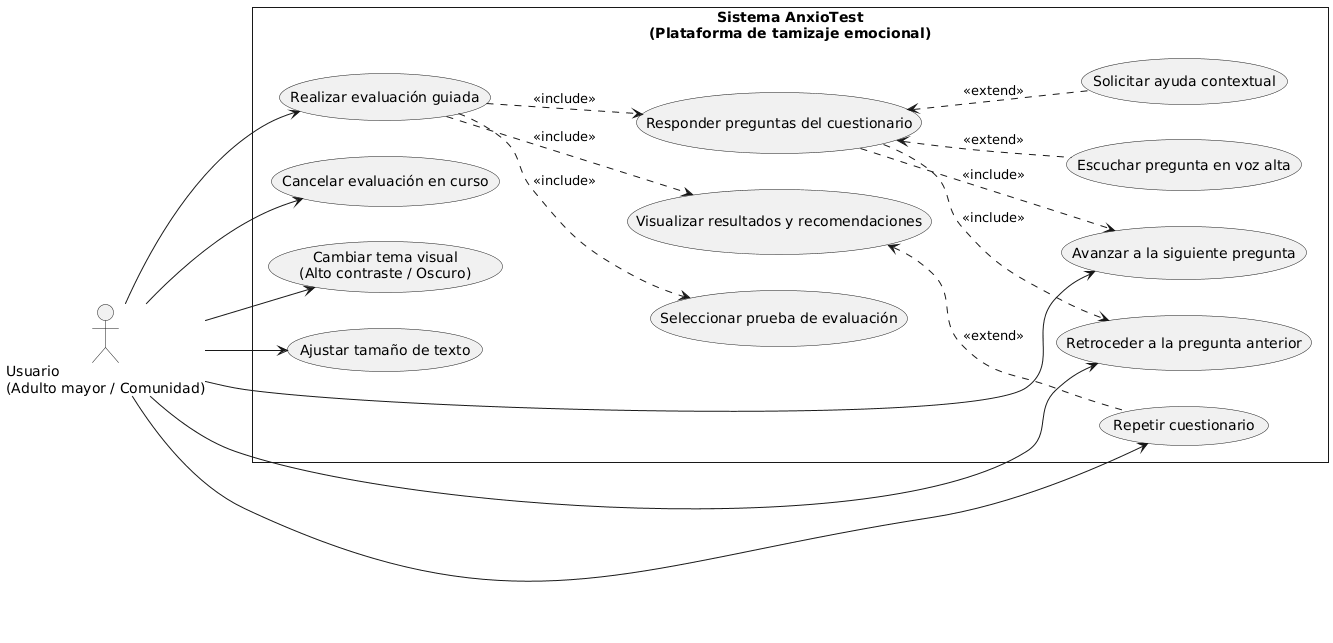
\includegraphics[width=0.9\textwidth]{nivel1-vincu.png}
  \caption{Diagrama de casos de uso – Nivel 1 (objetivos del usuario).}
  \label{fig:dcu_nivel1}
\end{figure}

\subsection{Listado de Casos de Uso Expandido (Nivel 1)}
\label{sec:casos_uso_expandido}

A continuación se detallan los casos de uso de nivel 1 que representan las interacciones concretas del usuario con el sistema. Cada caso de uso agrupa varios requisitos funcionales (RF) para mantener la trazabilidad.

\subsubsection{UC-01: Realizar evaluación guiada}

\begin{longtable}{p{0.22\linewidth} p{0.73\linewidth}}
\toprule
\rowcolor{tableheader!20}
\textbf{Campo} & \textbf{Detalle} \\
\midrule
\endfirsthead
\rowcolor{tableheader!20}
\textbf{Campo} & \textbf{Detalle} \\
\midrule
\endhead
\bottomrule
\endfoot
\textbf{Nombre del Requerimiento} & UC-01 -- Realizar evaluación guiada \\
\textbf{Descripción} & Permite al adulto mayor completar un cuestionario de tamizaje psicológico (PHQ-9 o BAI) de forma secuencial, una pregunta a la vez, con opciones de navegación (Siguiente / Anterior), cancelación y soporte de accesibilidad (teclado, ARIA). Este caso de uso es el núcleo del sistema e incluye la selección de prueba, el llenado del cuestionario y la visualización de resultados. \\
\textbf{Actor} & Usuario (Adulto mayor / Comunidad) \\
\textbf{Precondición} & El usuario dispone de un navegador moderno con JavaScript habilitado y ha accedido a la página de inicio de AnxioTest. \\
\textbf{Secuencia normal} & 
  \begin{enumerate}
    \item El Usuario accede a la página de bienvenida.
    \item El Usuario hace clic en ``Comenzar evaluación''.
    \item El Sistema muestra la página de selección de pruebas (PHQ-9 y BAI).
    \item El Usuario selecciona una prueba.
    \item El Sistema presenta la primera pregunta con 4 opciones de respuesta y un indicador de progreso.
    \item El Usuario selecciona una opción de respuesta.
    \item El Usuario pulsa el botón ``Siguiente''.
    \item El Sistema valida que haya una opción seleccionada, guarda la respuesta y avanza a la siguiente pregunta.
    \item Los pasos 5 a 8 se repiten hasta que el Usuario responde la última pregunta y pulsa ``Ver resultados''.
    \item El Sistema calcula el puntaje total, almacena el resultado en \texttt{sessionStorage} y redirige a la página de resultados.
  \end{enumerate} \\
\textbf{Postcondición} & El usuario ha completado todas las preguntas. Los resultados quedan almacenados temporalmente en el navegador para su visualización. \\
\textbf{Excepciones} & 
  \begin{itemize}
    \item \textbf{Paso 5:} El usuario pulsa ``Cancelar''. El Sistema muestra un diálogo de confirmación; si confirma, regresa al inicio perdiendo el progreso.
    \item \textbf{Paso 7:} El usuario intenta pulsar ``Siguiente'' sin seleccionar una opción. El Sistema mantiene el botón deshabilitado y no avanza.
  \end{itemize} \\
\textbf{Versión} & 1.0 \\
\textbf{Comentarios} & Este caso de uso incluye a \textbf{Seleccionar prueba de evaluación}, \textbf{Responder preguntas del cuestionario} y \textbf{Visualizar resultados y recomendaciones}. También se relaciona con \textbf{Cancelar evaluación en curso} y con las extensiones de \textbf{Solicitar ayuda contextual} y \textbf{Escuchar pregunta en voz alta}. \\
\bottomrule
\caption{Caso de uso expandido UC-01}
\label{tab:uc01}
\end{longtable}

\subsubsection{UC-02: Seleccionar prueba de evaluación}

\begin{longtable}{p{0.22\linewidth} p{0.73\linewidth}}
\toprule
\rowcolor{tableheader!20}
\textbf{Campo} & \textbf{Detalle} \\
\midrule
\endfirsthead
\rowcolor{tableheader!20}
\textbf{Campo} & \textbf{Detalle} \\
\midrule
\endhead
\bottomrule
\endfoot
\textbf{Nombre del Requerimiento} & UC-02 -- Seleccionar prueba de evaluación \\
\textbf{Descripción} & Permite al usuario elegir entre los dos cuestionarios disponibles: PHQ-9 (depresión) o BAI (ansiedad), desde la página de selección de pruebas. \\
\textbf{Actor} & Usuario (Adulto mayor / Comunidad) \\
\textbf{Precondición} & El usuario ha accedido a la página de selección de pruebas (después de hacer clic en ``Comenzar evaluación''). \\
\textbf{Secuencia normal} & 
  \begin{enumerate}
    \item El Sistema muestra dos tarjetas visuales: una para PHQ-9 y otra para BAI.
    \item El Usuario lee la descripción breve de cada cuestionario.
    \item El Usuario hace clic en el botón ``Iniciar'' o ``Realizar prueba'' de la tarjeta deseada.
    \item El Sistema redirige al usuario a la primera pregunta del cuestionario seleccionado.
  \end{enumerate} \\
\textbf{Postcondición} & El usuario ha iniciado el cuestionario elegido y se encuentra en la primera pregunta. \\
\textbf{Excepciones} & 
  \begin{itemize}
    \item \textbf{Paso 3:} El usuario hace clic en ``Volver al inicio'' en lugar de seleccionar una prueba; el sistema regresa a la página principal.
  \end{itemize} \\
\textbf{Versión} & 1.0 \\
\textbf{Comentarios} & Este caso de uso cubre los RF-2, RF-3 y RF-4. Es incluido por UC-01 (Realizar evaluación guiada). \\
\bottomrule
\caption{Caso de uso expandido UC-02}
\label{tab:uc02}
\end{longtable}

\subsubsection{UC-03: Responder preguntas del cuestionario}

\begin{longtable}{p{0.22\linewidth} p{0.73\linewidth}}
\toprule
\rowcolor{tableheader!20}
\textbf{Campo} & \textbf{Detalle} \\
\midrule
\endfirsthead
\rowcolor{tableheader!20}
\textbf{Campo} & \textbf{Detalle} \\
\midrule
\endhead
\bottomrule
\endfoot
\textbf{Nombre del Requerimiento} & UC-03 -- Responder preguntas del cuestionario \\
\textbf{Descripción} & Permite al usuario avanzar a través de las preguntas del cuestionario, seleccionando una opción de respuesta por cada pregunta, y navegar entre ellas con los botones ``Siguiente'' y ``Anterior''. \\
\textbf{Actor} & Usuario (Adulto mayor / Comunidad) \\
\textbf{Precondición} & El usuario ha seleccionado un cuestionario (UC-02) y se encuentra en la primera pregunta. \\
\textbf{Secuencia normal} & 
  \begin{enumerate}
    \item El Sistema muestra la pregunta actual con cuatro opciones de respuesta y un indicador de progreso (número de pregunta y porcentaje).
    \item El Usuario selecciona una opción de respuesta.
    \item El Usuario pulsa el botón ``Siguiente'' para avanzar (o ``Anterior'' para retroceder).
    \item El Sistema valida que haya una opción seleccionada (para ``Siguiente''), guarda la respuesta y muestra la siguiente pregunta (o la anterior).
    \item El proceso se repite hasta llegar a la última pregunta, donde el botón ``Siguiente'' cambia a ``Ver resultados''.
  \end{enumerate} \\
\textbf{Postcondición} & El usuario ha respondido todas las preguntas y está listo para ver los resultados. \\
\textbf{Excepciones} & 
  \begin{itemize}
    \item \textbf{Paso 3:} El usuario intenta pulsar ``Siguiente'' sin seleccionar una opción. El Sistema mantiene el botón deshabilitado y no avanza.
    \item \textbf{Paso 3:} El usuario pulsa ``Cancelar''; el Sistema muestra un diálogo de confirmación y, si se confirma, regresa al inicio.
  \end{itemize} \\
\textbf{Versión} & 1.0 \\
\textbf{Comentarios} & Este caso de uso cubre los RF-5, RF-6, RF-7, RF-8, RF-9, RF-10 y RF-13. Es incluido por UC-01 y puede extenderse con UC-06 (Solicitar ayuda contextual) y UC-07 (Escuchar pregunta en voz alta). \\
\bottomrule
\caption{Caso de uso expandido UC-03}
\label{tab:uc03}
\end{longtable}

\subsubsection{UC-04: Visualizar resultados y recomendaciones}

\begin{longtable}{p{0.22\linewidth} p{0.73\linewidth}}
\toprule
\rowcolor{tableheader!20}
\textbf{Campo} & \textbf{Detalle} \\
\midrule
\endfirsthead
\rowcolor{tableheader!20}
\textbf{Campo} & \textbf{Detalle} \\
\midrule
\endhead
\bottomrule
\endfoot
\textbf{Nombre del Requerimiento} & UC-04 -- Visualizar resultados y recomendaciones \\
\textbf{Descripción} & Permite al usuario conocer el puntaje obtenido, la categoría de severidad (con un lenguaje amigable y no alarmista) y recibir recomendaciones prácticas de autocuidado o derivación profesional. \\
\textbf{Actor} & Usuario (Adulto mayor / Comunidad) \\
\textbf{Precondición} & El usuario ha completado todas las preguntas del cuestionario (UC-03) y ha pulsado ``Ver resultados''. El sistema ha almacenado el resultado en \texttt{sessionStorage}. \\
\textbf{Secuencia normal} & 
  \begin{enumerate}
    \item El Sistema carga la página de resultados.
    \item El Sistema recupera los datos de \texttt{sessionStorage}.
    \item El Sistema muestra el puntaje numérico, la categoría de severidad (ej. ``Algunos días pesan más que otros'') y un mensaje interpretativo personalizado.
    \item El Sistema presenta una lista de recomendaciones prácticas adaptadas al nivel de severidad.
    \item El Sistema muestra los botones ``Repetir cuestionario'' y ``Volver al inicio''.
    \item El Usuario lee la información proporcionada.
  \end{enumerate} \\
\textbf{Postcondición} & El usuario comprende su nivel de bienestar emocional y dispone de orientación sobre los pasos a seguir. \\
\textbf{Excepciones} & 
  \begin{itemize}
    \item \textbf{Paso 2:} No hay datos en \texttt{sessionStorage}. El Sistema muestra un mensaje ``No hay resultados disponibles'' y ofrece un botón para volver al inicio.
  \end{itemize} \\
\textbf{Versión} & 1.0 \\
\textbf{Comentarios} & Este caso de uso cubre los RF-14, RF-15, RF-16, RF-17, RF-18, RF-19, RF-20, RF-21, RF-26 y RF-27. Es incluido por UC-01 e incluye a UC-10 (Repetir cuestionario). \\
\bottomrule
\caption{Caso de uso expandido UC-04}
\label{tab:uc04}
\end{longtable}

\subsubsection{UC-05: Cancelar evaluación en curso}

\begin{longtable}{p{0.22\linewidth} p{0.73\linewidth}}
\toprule
\rowcolor{tableheader!20}
\textbf{Campo} & \textbf{Detalle} \\
\midrule
\endfirsthead
\rowcolor{tableheader!20}
\textbf{Campo} & \textbf{Detalle} \\
\midrule
\endhead
\bottomrule
\endfoot
\textbf{Nombre del Requerimiento} & UC-05 -- Cancelar evaluación en curso \\
\textbf{Descripción} & Permite al usuario interrumpir el cuestionario en cualquier momento, mostrando un diálogo de confirmación para evitar cancelaciones accidentales. \\
\textbf{Actor} & Usuario (Adulto mayor / Comunidad) \\
\textbf{Precondición} & El usuario se encuentra respondiendo preguntas del cuestionario (dentro de UC-03). \\
\textbf{Secuencia normal} & 
  \begin{enumerate}
    \item El Usuario identifica el botón ``Cancelar'' en la página del cuestionario.
    \item El Usuario hace clic en ``Cancelar''.
    \item El Sistema muestra un diálogo de confirmación con las opciones: ``Sí, cancelar'' y ``Continuar''.
    \item El Usuario selecciona ``Sí, cancelar''.
    \item El Sistema descarta el progreso actual y redirige al usuario a la página de inicio.
  \end{enumerate} \\
\textbf{Postcondición} & La evaluación se cancela y el usuario vuelve a la página de inicio sin guardar respuestas. \\
\textbf{Excepciones} & 
  \begin{itemize}
    \item \textbf{Paso 4:} El Usuario selecciona ``Continuar''; el diálogo se cierra y el usuario regresa a la pregunta actual sin perder el progreso.
  \end{itemize} \\
\textbf{Versión} & 1.0 \\
\textbf{Comentarios} & Este caso de uso cubre el RF-13. Es independiente pero se activa desde UC-03. \\
\bottomrule
\caption{Caso de uso expandido UC-05}
\label{tab:uc05}
\end{longtable}

\subsubsection{UC-06: Solicitar ayuda contextual}

\begin{longtable}{p{0.22\linewidth} p{0.73\linewidth}}
\toprule
\rowcolor{tableheader!20}
\textbf{Campo} & \textbf{Detalle} \\
\midrule
\endfirsthead
\rowcolor{tableheader!20}
\textbf{Campo} & \textbf{Detalle} \\
\midrule
\endhead
\bottomrule
\endfoot
\textbf{Nombre del Requerimiento} & UC-06 -- Solicitar ayuda contextual \\
\textbf{Descripción} & Permite al usuario obtener información adicional sobre la pregunta actual, el cuestionario en general o el significado de las opciones de respuesta, mediante un modal informativo. \\
\textbf{Actor} & Usuario (Adulto mayor / Comunidad) \\
\textbf{Precondición} & El usuario se encuentra respondiendo una pregunta del cuestionario (UC-03). \\
\textbf{Secuencia normal} & 
  \begin{enumerate}
    \item El Usuario identifica el botón de ayuda (icono de interrogación) junto a la pregunta.
    \item El Usuario hace clic en el botón.
    \item El Sistema muestra un modal con información contextual relevante (descripción del cuestionario, aclaración de la pregunta, significado de las opciones).
    \item El Usuario lee la información.
    \item El Usuario cierra el modal (clic en ``Cerrar'' o fuera del modal) y regresa a la pregunta.
  \end{enumerate} \\
\textbf{Postcondición} & El usuario ha recibido información adicional que le ayuda a comprender mejor la pregunta. \\
\textbf{Excepciones} & Ninguna. \\
\textbf{Versión} & 1.0 \\
\textbf{Comentarios} & Este caso de uso cubre el RF-12. Es una extensión de UC-03 (Responder preguntas del cuestionario). \\
\bottomrule
\caption{Caso de uso expandido UC-06}
\label{tab:uc06}
\end{longtable}

\subsubsection{UC-07: Escuchar pregunta en voz alta}

\begin{longtable}{p{0.22\linewidth} p{0.73\linewidth}}
\toprule
\rowcolor{tableheader!20}
\textbf{Campo} & \textbf{Detalle} \\
\midrule
\endfirsthead
\rowcolor{tableheader!20}
\textbf{Campo} & \textbf{Detalle} \\
\midrule
\endhead
\bottomrule
\endfoot
\textbf{Nombre del Requerimiento} & UC-07 -- Escuchar pregunta en voz alta \\
\textbf{Descripción} & Permite al usuario activar la síntesis de voz (Text-to-Speech) para que el navegador lea en voz alta la pregunta actual y sus opciones de respuesta, facilitando la comprensión a personas con dificultades visuales o de lectura. \\
\textbf{Actor} & Usuario (Adulto mayor / Comunidad) \\
\textbf{Precondición} & El usuario se encuentra respondiendo una pregunta del cuestionario (UC-03). El navegador soporta la API \texttt{SpeechSynthesis}. \\
\textbf{Secuencia normal} & 
  \begin{enumerate}
    \item El Usuario identifica el botón de lectura por voz (ícono de altavoz) junto a la pregunta.
    \item El Usuario hace clic en el botón.
    \item El Sistema detiene cualquier reproducción de voz en curso.
    \item El Sistema utiliza la API \texttt{SpeechSynthesis} del navegador para generar la voz.
    \item El Sistema lee en voz alta el texto de la pregunta y, a continuación, las 4 opciones de respuesta.
    \item El Sistema finaliza la lectura.
  \end{enumerate} \\
\textbf{Postcondición} & El usuario ha escuchado la pregunta y las opciones, lo que le permite tomar una decisión de respuesta con mayor comprensión. \\
\textbf{Excepciones} & 
  \begin{itemize}
    \item \textbf{Paso 3:} El navegador no soporta la API TTS. El Sistema oculta el botón o muestra un mensaje de ``Función no disponible''.
    \item \textbf{Paso 4:} La voz sintetizada no es clara. El sistema usa la voz predeterminada del navegador (configurable por el usuario en su SO).
  \end{itemize} \\
\textbf{Versión} & 1.0 \\
\textbf{Comentarios} & Este caso de uso cubre el RF-11 y los requisitos de accesibilidad (RNF-14 a RNF-18). Es una extensión de UC-03. \\
\bottomrule
\caption{Caso de uso expandido UC-07}
\label{tab:uc07}
\end{longtable}

\subsubsection{UC-08: Cambiar tema visual}

\begin{longtable}{p{0.22\linewidth} p{0.73\linewidth}}
\toprule
\rowcolor{tableheader!20}
\textbf{Campo} & \textbf{Detalle} \\
\midrule
\endfirsthead
\rowcolor{tableheader!20}
\textbf{Campo} & \textbf{Detalle} \\
\midrule
\endhead
\bottomrule
\endfoot
\textbf{Nombre del Requerimiento} & UC-08 -- Cambiar tema visual \\
\textbf{Descripción} & Permite al usuario seleccionar entre diferentes esquemas de colores predefinidos (Claro, Oscuro, Alto Contraste) para adaptar la apariencia del sistema a sus necesidades visuales. \\
\textbf{Actor} & Usuario (Adulto mayor / Comunidad) \\
\textbf{Precondición} & El usuario ha accedido al sistema y se encuentra en cualquier página (inicio, selección, cuestionario o resultados). \\
\textbf{Secuencia normal} & 
  \begin{enumerate}
    \item El Usuario localiza el selector de temas en el encabezado de la página.
    \item El Usuario despliega las opciones disponibles (Claro, Oscuro, Alto Contraste).
    \item El Usuario selecciona una opción.
    \item El Sistema aplica el tema seleccionado de inmediato a toda la interfaz.
    \item El Sistema guarda la preferencia en \texttt{localStorage} para futuras visitas.
  \end{enumerate} \\
\textbf{Postcondición} & La interfaz del sistema se muestra con el tema visual elegido por el usuario. \\
\textbf{Excepciones} & Ninguna. \\
\textbf{Versión} & 1.0 \\
\textbf{Comentarios} & Este caso de uso cubre los RF-22 y RF-23. Es independiente y puede ejecutarse en cualquier momento. \\
\bottomrule
\caption{Caso de uso expandido UC-08}
\label{tab:uc08}
\end{longtable}

\subsubsection{UC-09: Ajustar tamaño de texto}

\begin{longtable}{p{0.22\linewidth} p{0.73\linewidth}}
\toprule
\rowcolor{tableheader!20}
\textbf{Campo} & \textbf{Detalle} \\
\midrule
\endfirsthead
\rowcolor{tableheader!20}
\textbf{Campo} & \textbf{Detalle} \\
\midrule
\endhead
\bottomrule
\endfoot
\textbf{Nombre del Requerimiento} & UC-09 -- Ajustar tamaño de texto \\
\textbf{Descripción} & Permite al usuario modificar el tamaño de la fuente mediante los controles del navegador (zoom o ajuste de fuente), sin que el diseño se rompa. \\
\textbf{Actor} & Usuario (Adulto mayor / Comunidad) \\
\textbf{Precondición} & El usuario ha accedido al sistema y se encuentra en cualquier página. \\
\textbf{Secuencia normal} & 
  \begin{enumerate}
    \item El Usuario utiliza los controles nativos del navegador (Ctrl+ / Ctrl- o menú de zoom).
    \item El navegador escala el contenido.
    \item El Sistema mantiene la legibilidad y funcionalidad sin superposición de elementos ni pérdida de información.
  \end{enumerate} \\
\textbf{Postcondición} & El texto se muestra en un tamaño más grande o más pequeño, según la preferencia del usuario. \\
\textbf{Excepciones} & 
  \begin{itemize}
    \item El sistema no debe romperse ni ocultar contenido al aplicar zoom hasta el 200\,\%.
  \end{itemize} \\
\textbf{Versión} & 1.0 \\
\textbf{Comentarios} & Este caso de uso no requiere un botón específico en la interfaz; se apoya en las capacidades del navegador. Cubre el RNF-17 y parte de los requisitos de accesibilidad. \\
\bottomrule
\caption{Caso de uso expandido UC-09}
\label{tab:uc09}
\end{longtable}

\subsubsection{UC-10: Repetir cuestionario}

\begin{longtable}{p{0.22\linewidth} p{0.73\linewidth}}
\toprule
\rowcolor{tableheader!20}
\textbf{Campo} & \textbf{Detalle} \\
\midrule
\endfirsthead
\rowcolor{tableheader!20}
\textbf{Campo} & \textbf{Detalle} \\
\midrule
\endhead
\bottomrule
\endfoot
\textbf{Nombre del Requerimiento} & UC-10 -- Repetir cuestionario \\
\textbf{Descripción} & Permite al usuario reiniciar el mismo cuestionario después de haber visto los resultados, sin necesidad de volver a la página de selección. \\
\textbf{Actor} & Usuario (Adulto mayor / Comunidad) \\
\textbf{Precondición} & El usuario ha visualizado los resultados de un cuestionario (UC-04) y se encuentra en la página de resultados. \\
\textbf{Secuencia normal} & 
  \begin{enumerate}
    \item El Usuario identifica el botón ``Repetir cuestionario'' en la página de resultados.
    \item El Usuario hace clic en el botón.
    \item El Sistema reinicia el cuestionario, mostrando la primera pregunta del mismo test.
    \item El Usuario puede volver a responder las preguntas.
  \end{enumerate} \\
\textbf{Postcondición} & El usuario comienza nuevamente el cuestionario, con todas las respuestas reiniciadas. \\
\textbf{Excepciones} & Ninguna. \\
\textbf{Versión} & 1.0 \\
\textbf{Comentarios} & Este caso de uso cubre el RF-21. Es incluido por UC-04 (Visualizar resultados). \\
\bottomrule
\caption{Caso de uso expandido UC-10}
\label{tab:uc10}
\end{longtable}

\subsubsection{UC-11: Retroceder a la pregunta anterior}

\begin{longtable}{p{0.22\linewidth} p{0.73\linewidth}}
\toprule
\rowcolor{tableheader!20}
\textbf{Campo} & \textbf{Detalle} \\
\midrule
\endfirsthead
\rowcolor{tableheader!20}
\textbf{Campo} & \textbf{Detalle} \\
\midrule
\endhead
\bottomrule
\endfoot
\textbf{Nombre del Requerimiento} & UC-11 -- Retroceder a la pregunta anterior \\
\textbf{Descripción} & Permite al usuario volver a una pregunta previa del cuestionario para revisar o modificar su respuesta. \\
\textbf{Actor} & Usuario (Adulto mayor / Comunidad) \\
\textbf{Precondición} & El usuario se encuentra en una pregunta del cuestionario (UC-03) que no es la primera (es decir, ha avanzado al menos una pregunta). \\
\textbf{Secuencia normal} & 
  \begin{enumerate}
    \item El Usuario identifica el botón ``Anterior'' en la página del cuestionario.
    \item El Usuario hace clic en el botón.
    \item El Sistema muestra la pregunta anterior, manteniendo la opción que el usuario había seleccionado previamente.
    \item El Usuario puede modificar su respuesta si lo desea.
  \end{enumerate} \\
\textbf{Postcondición} & El usuario se encuentra en la pregunta anterior y puede cambiar su respuesta. \\
\textbf{Excepciones} & 
  \begin{itemize}
    \item El botón ``Anterior'' está deshabilitado en la primera pregunta.
  \end{itemize} \\
\textbf{Versión} & 1.0 \\
\textbf{Comentarios} & Este caso de uso cubre el RF-9. Es parte de UC-03 (Responder preguntas). \\
\bottomrule
\caption{Caso de uso expandido UC-11}
\label{tab:uc11}
\end{longtable}

\subsection{Relación de casos de uso con requisitos funcionales}
\label{sec:trazabilidad_casos}

La siguiente tabla resume la cobertura de los requisitos funcionales (RF) por cada caso de uso expandido:

\begin{longtable}{p{0.25\linewidth} p{0.70\linewidth}}
\toprule
\rowcolor{tableheader!20}
\textbf{Caso de Uso} & \textbf{Requisitos funcionales cubiertos} \\
\midrule
\endfirsthead
\rowcolor{tableheader!20}
\textbf{Caso de Uso} & \textbf{Requisitos funcionales cubiertos} \\
\midrule
\endhead
\bottomrule
\endfoot
UC-01: Realizar evaluación guiada & (Aglutina los demás casos de uso) \\
UC-02: Seleccionar prueba de evaluación & RF-2, RF-3, RF-4 \\
UC-03: Responder preguntas del cuestionario & RF-5, RF-6, RF-7, RF-8, RF-9, RF-10 \\
UC-04: Visualizar resultados y recomendaciones & RF-14, RF-15, RF-16, RF-17, RF-18, RF-19, RF-20, RF-21, RF-26, RF-27 \\
UC-05: Cancelar evaluación en curso & RF-13 \\
UC-06: Solicitar ayuda contextual & RF-12 \\
UC-07: Escuchar pregunta en voz alta & RF-11 \\
UC-08: Cambiar tema visual & RF-22, RF-23 \\
UC-09: Ajustar tamaño de texto & RNF-17 (no es RF, pero se menciona) \\
UC-10: Repetir cuestionario & RF-21 \\
UC-11: Retroceder a la pregunta anterior & RF-9 \\
\bottomrule
\caption{Trazabilidad casos de uso -- requisitos funcionales}
\label{tab:trazabilidad}
\end{longtable}

\textbf{Nota:} Los requisitos funcionales RF-1 (Pantalla de bienvenida), RF-24 (Navegación por teclado) y RF-25 (Atributos ARIA) son transversales y se aplican a todos los casos de uso; por lo tanto, no se asignan a un caso específico. El RF-1 es la página de inicio que da acceso a todo el sistema.